

\subsection{Distros}
\begin{frame}
\frametitle{Was ist eine Dist.?}
Betrieben von Community/Firmen.
Kümmern sich um: 
\begin{itemize}
 \item Pakete
 \item Änderungen/Patches
 \item Hilfe/Support
\end{itemize}
 
\end{frame}

\begin{frame}
 \frametitle{Vorkommen}

 
 \begin{itemize}
  \item Raspian/Kodi/..
  \item Android/Sailfish
  \item Alpine/TinyCore/CoreOS
  \item viele embedded Geräte mit speziell angepasstem Linux
 (wie Router, Steuergeräte, Mediengeräte)
 \end{itemize}

\end{frame}



\begin{frame}
\frametitle{Bsp. Distros}
\begin{itemize}%[<+->]
\item Debian
\item Ubuntu
\item Mint
\item Arch
\item openSuse
\item RHEL/Fedora/CentOS 
\item gentoo
\item Puppy/Knoppix 

\item Kali 

\end{itemize}
\end{frame}

\subsection{Oberflächen}
\begin{frame}
\frametitle{Oberflächen}

\begin{multicols}{2}
\onslide<1->{\begin{figure}
 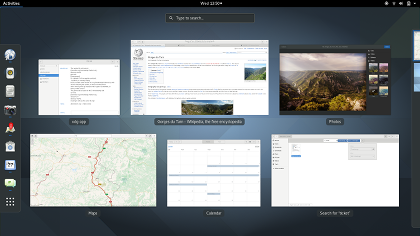
\includegraphics[width=0.45\textwidth]{resources/window-selection.png}
%\footnote{https://www.gnome.org/wp-content/uploads/2016/03/window-selection-3.20-420x236.png}
 \end{figure}
}
\onslide<2->{

\begin{figure}
 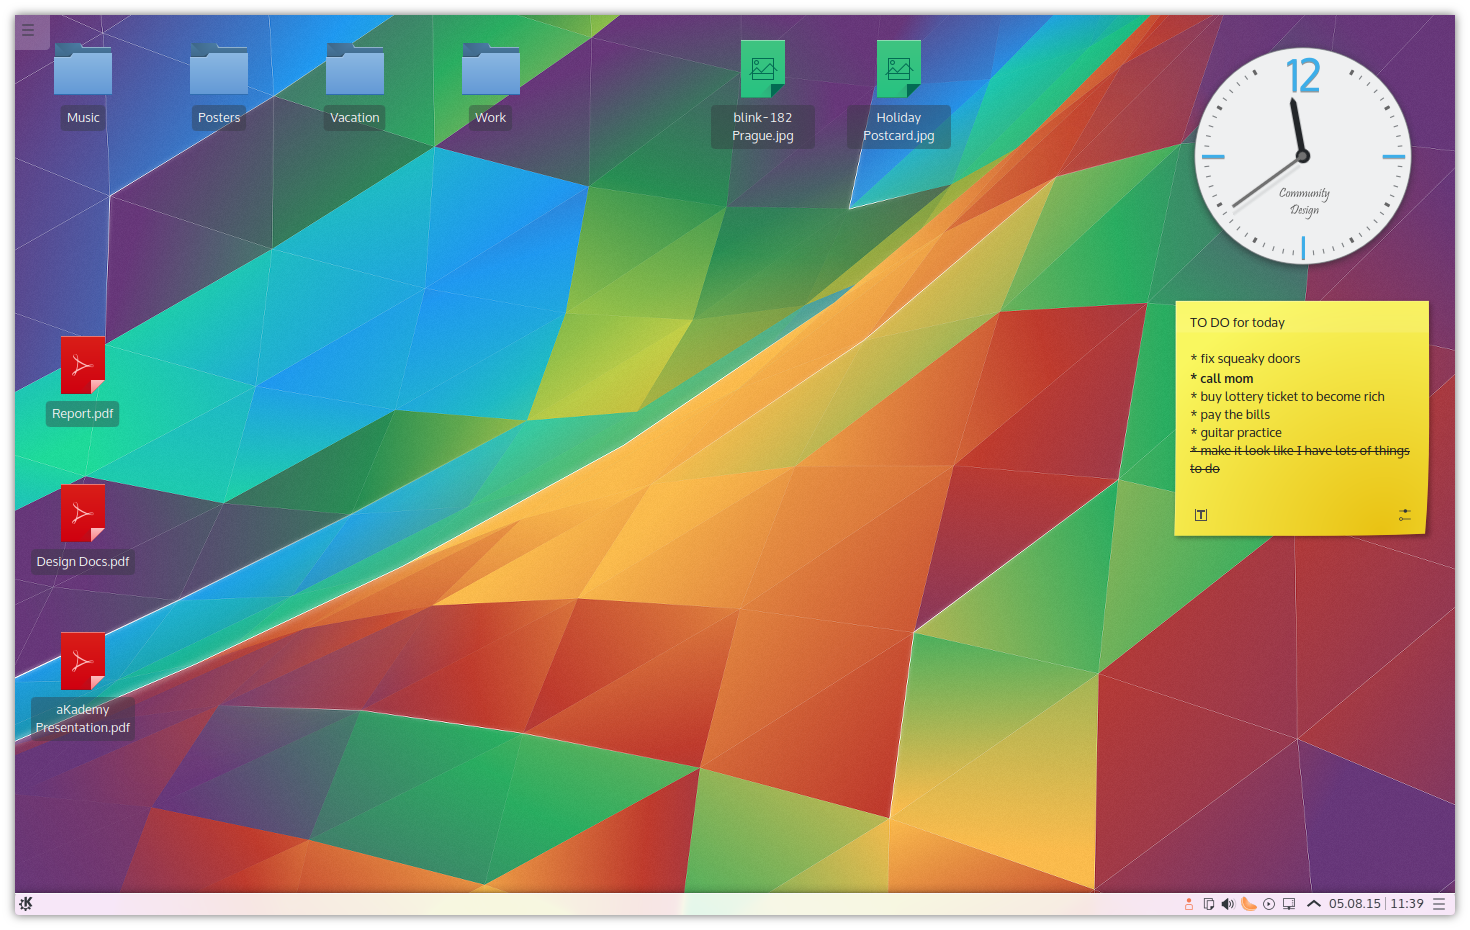
\includegraphics[width=0.45\textwidth]{resources/general-desktop.png}
\end{figure}
%\footnote{https://www.kde.org/workspaces/plasmadesktop/screenshots/general-desktop.png}
}


\only<1>{Gnome}
\only<2>{KDE: Plasma}
\only<3>{Unity (Ubuntu)}
\onslide<4>{\begin{figure}
  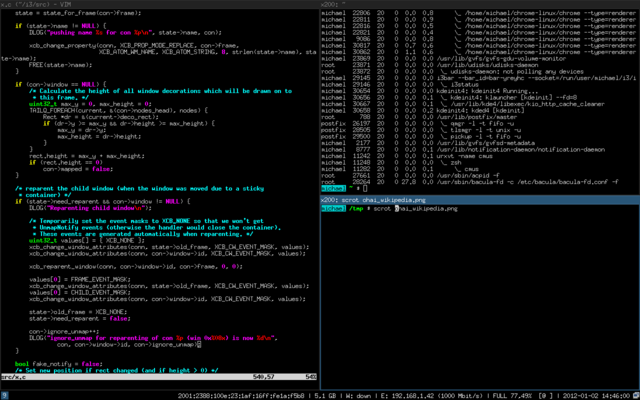
\includegraphics[width=0.45\textwidth]{resources/I3_window_manager_screenshot.png} %Nammensnennung!!
  %footnote{https://de.wikipedia.org/wiki/I3_(Fenstermanager)#/media/File:I3_window_manager_screenshot.png}
  \end{figure}
  
  \onslide<3->{\begin{figure}
  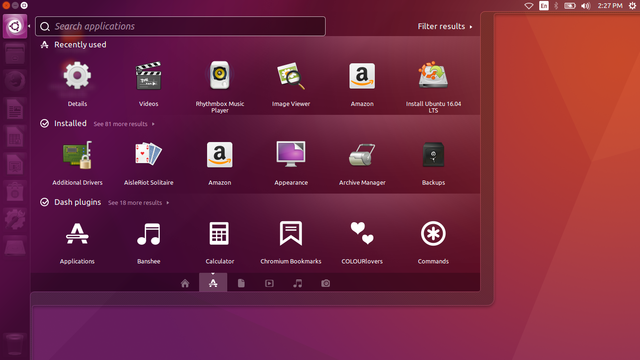
\includegraphics[width=0.45\textwidth]{resources/App_Lens_on_Ubuntu_16.png}
 %\footnote{https://en.wikipedia.org/wiki/Unity_(user_interface)#/media/File:App_Lens_on_Ubuntu_16.04LTS.png}
\end{figure}}
}

%\begin{itemize}
%\item Gnome3
%\item KDE
%\item mate
%\item Konsole
%\end{itemize}

\end{multicols}

\end{frame}


\subsection{Programme}
\begin{frame}[allowframebreaks]
 \frametitle{Programme}
 %\begin{tabular}{lp{5cm}}
 %Kategorie& Software \\ \hline
 
\hspace{1cm}

\begin{description}[style=nextline]

\item [ Browser] {\bf Firefox}, Chromium, Vivaldi, Tor, Lynx
% \item  Chromium
% \item  Lynx
% \item  Opera bzw. Vivaldi
% \item  Safari
% \item  Tor Browser 
%  \end{category}
\item [Office] LibreOffice, Kile (\LaTeX), \TeX maker
% \item Kile (\LaTeX)
% \item \TeX maker 
% \item TeXstudio 
% \item Brasero 
% \end{category}
 \item [Email Clients ] Thunderbird, Icedove, Evolution 
% \item Icedove 
% \item Evolution 
% %  \end{category}
 \item [IDEs] Eclipse, IntelliJ, NetBeans, Atom, VI(M)
% \item IntelliJ 
% \item NetBeans 
% \item QtCreator 
% \item Atom 
% \item Bluefish 
% \item VI(M)  
% % \end{category}
 \item  [Musik] VLC, Rythmbox, Amarok 
% \item Banshee 
% \item Rythmbox 
% \item DragonPlayer 
% \item Amarok 
% %  \end{category}
 \item  [Videos] VLC, Totem
% \item Totem ??? 
% %  \end{category}
 \item  [Medien] GIMP, Blender, Audacity, Inkscape
% \item Inkscape 
% \item Blender 
% \item Audacity 
% \item KDEnlive 
% \item AviDeMux 
% %\end{category}
 \item  [Messenger] Pidgin, Empathy, HexChat, Telegram
% \item Pidgin 
% \item Empathy 
% \item HexChat 
% \item WeeChat 
% \item Telegram 
% \item Matrix-Clients 
% %  \end{category}
 \item  [VoIP] Mumble, Ring, Tox
% \item Ekiga 
% \item Ring 
% \item Tox 
% %  \end{category}
 \item  [System] GParted, Wireshark, Boabab, Filezilla
% \item Wireshark 
% \item Htop 
% \item Boabab 
% \item Tor 
% \item OpenVPN 
% \item Filezilla 
% %  \end{category}
 \item  [  Torrents] Transmission 
% % \end{category}
 \item  [Synchronisation] Nextcloud, Owncloud, Seafile
% \item Owncloud 
% \item Seafile 
 \item   [alles] DAS TERMINAL 
 %\end{tabular}
\end{description}
 \end{frame}




